%%%%%%%%%%%%%%%%%%%%%%%%%%%%%%%%%%%%%%%%%%%%%%%%%%%%%%%%%%%%%%%%%%%%%%%%%%%%%%%%%%%%
% Configuración de Paquetes
\documentclass{article}
\usepackage[framemethod=TikZ]{mdframed}
\usepackage{booktabs}
\usepackage{float}
\usepackage{scrextend}
\usepackage{titletoc}
\usepackage[margin=1in]{geometry} 
\usepackage{amsmath,amsthm,amssymb,amsfonts, fancyhdr, color, comment, graphicx, environ}
\usepackage{xcolor}
\usepackage{mdframed}
\usepackage[shortlabels]{enumitem}
\usepackage{indentfirst}
\usepackage{hyperref}
\usepackage{listings}
\usepackage{tikz}
\usepackage[framemethod=TikZ]{mdframed}
\usepackage{mathptmx}
\usepackage{cfr-lm}
\usepackage{color}
\hypersetup{
    colorlinks=true,
    linkcolor=blue,
    filecolor=magenta,      
    urlcolor=blue,
}
\setlength{\headheight}{1.5cm}
\renewcommand{\qed}{\quad\qedsymbol}
\usetikzlibrary{calc}
\renewcommand{\familydefault}{\sfdefault}
%%%%%%%%%%%%%%%%%%%%%%%%%%%%%%%%%%%%%%%%%%%%%%%%%%%%%%%%%%%%%%%%%%%%%%%%%%%%%%%%%%%%

\fancypagestyle{mipagina}{
    \fancyhf{} % Limpiar encabezado y pie de página
    \fancyhead[L]{Pedro Villar} % Nombre a la izquierda
    \fancyhead[C]{\rightmark} % Texto al centro 
    \fancyhead[R]{Org. del Computador} % Texto a la derecha
    \fancyfoot[C]{\thepage} % Número de página al centro
    \renewcommand{\headrulewidth}{0.4pt} % Grosor de la línea horizontal en el encabezado
}

\pagestyle{mipagina}
\mdfsetup{skipabove=\topskip,skipbelow=\topskip}

% Box de Definición
\newcounter{def}[section]

\NewDocumentEnvironment{defi}{o}{%
    \stepcounter{def}%
    \begin{mdframed}[
        frametitle={%
            \begin{tikzpicture}[baseline=(current bounding box.east),outer sep=0pt]
                \node[anchor=east,rectangle,fill=blue!20,inner xsep=5pt] at (0,0) {\strut\IfValueTF{#1}{Definición~\thedef:~#1}{Definición~\thedef}};
            \end{tikzpicture}%
        },
        innertopmargin=5pt,
        linecolor=blue!20,
        linewidth=2pt,
        topline=true,
        frametitleaboveskip=-\ht\strutbox, % Ajuste de espacio entre título y contenido
        frametitlealignment={\hspace{5pt}}, % Ajuste de espacio entre el borde del frame y el título
    ]
}{%
    \end{mdframed}%
}

% Box de ejemplos
\newcounter{ejemplo}[section]

\NewDocumentEnvironment{ejemplo}{o}{%
    \stepcounter{ejemplo}%
    \begin{mdframed}[
        frametitle={%
            \begin{tikzpicture}[baseline=(current bounding box.east),outer sep=0pt]
                \node[anchor=east,rectangle,fill=brown!30,inner xsep=5pt] at (0,0) {\strut\IfValueTF{#1}{Ejemplo~\theejemplo:~#1}{Ejemplo~\theejemplo}};
            \end{tikzpicture}%
        },
        innertopmargin=5pt,
        linecolor=brown!30,
        linewidth=2pt,
        topline=true,
        frametitleaboveskip=-\ht\strutbox, % Ajuste de espacio entre título y contenido
        frametitlealignment={\hspace{5pt}}, % Ajuste de espacio entre el borde del frame y el título
    ]
}{%
    \end{mdframed}%
}

% Entorno para Métodos (color verde)
\newcounter{metodo}[section]
\NewDocumentEnvironment{metodo}{o}{%
    \stepcounter{metodo}%
    \begin{mdframed}[
        frametitle={%
            \begin{tikzpicture}[baseline=(current bounding box.east),outer sep=0pt]
                \node[anchor=east,rectangle,fill=green!30,inner xsep=5pt] at (0,0) {\strut\IfValueTF{#1}{Método~\themetodo:~#1}{Método~\themetodo}};
            \end{tikzpicture}%
        },
        innertopmargin=5pt,
        linecolor=green!30,
        linewidth=2pt,
        topline=true,
        frametitleaboveskip=-\ht\strutbox, % Ajuste de espacio entre título y contenido
        frametitlealignment={\hspace{5pt}}, % Ajuste de espacio entre el borde del frame y el título
    ]
}{%
    \end{mdframed}%
}

% Entorno para Observaciones (color amarillo más oscuro)
\newcounter{observacion}[section]
\NewDocumentEnvironment{observacion}{o}{%
    \stepcounter{observacion}%
    \begin{mdframed}[
        frametitle={%
            \begin{tikzpicture}[baseline=(current bounding box.east),outer sep=0pt]
                \node[anchor=east,rectangle,fill=yellow!50,inner xsep=5pt] at (0,0) {\strut\IfValueTF{#1}{Observación~\theobservacion:~#1}{Observación~\theobservacion}};
            \end{tikzpicture}%
        },
        innertopmargin=5pt,
        linecolor=yellow!50,
        linewidth=2pt,
        topline=true,
        frametitleaboveskip=-\ht\strutbox, % Ajuste de espacio entre título y contenido
        frametitlealignment={\hspace{5pt}}, % Ajuste de espacio entre el borde del frame y el título
    ]
}{%
    \end{mdframed}%
}

% Entorno para Ejercicio
\newcounter{ejer}[section]
\NewDocumentEnvironment{ejer}{o}{%
    \stepcounter{ejer}%
    \begin{mdframed}[
        frametitle={%
            \begin{tikzpicture}[baseline=(current bounding box.east),outer sep=0pt]
                \node[anchor=east,rectangle,fill=black!30,inner xsep=5pt] at (0,0) {\strut\IfValueTF{#1}{Ejercicio~\theejer:~#1}{Ejercicio~\theejer}};
            \end{tikzpicture}%
        },
        innertopmargin=5pt,
        linecolor=black!30,
        linewidth=2pt,
        topline=true,
        frametitleaboveskip=-\ht\strutbox, % Ajuste de espacio entre título y contenido
        frametitlealignment={\hspace{5pt}}, % Ajuste de espacio entre el borde del frame y el título
    ]
}{%
    \end{mdframed}%
}

\newenvironment{solution}
    {\textit{Solución:}}
    {}

%Configuraciones adicionales
\binoppenalty=\maxdimen 
\relpenalty=\maxdimen 
\setlength{\parindent}{0pt}

\begin{document}

\section*{Ejercicio 1}
Simplificar las siguientes funciones booleanas a un número mínimo de literales.
\begin{enumerate}[a)]
    \item $x \cdot y + x \cdot y'$
    \item $ ( x + y ) \cdot ( x + y')$
    \item $ x\cdot y \cdot z + x' \cdot y + x \cdot y \cdot z'$
    \item $z \cdot x + z \cdot x' \cdot y$
    \item $ (A+B)' \cdot (A' + B')'$
    \item $ y \cdot (w \cdot z' + w \cdot z) + x \cdot y $
\end{enumerate}

\begin{solution}
\textbf{Punto a)}\\
La función $x \cdot y + x \cdot y'$ se puede simplificar de la siguiente manera:
\begin{align*}
    x \cdot y + x \cdot y' &= x \cdot (y + y') (\text{postulado 4.}) \\
    &= x \cdot 1 (\text{postulado 5.}) \\
    &= x (\text{postulado 2.})
\end{align*}

\textbf{Punto b)}\\
La función $( x + y ) \cdot ( x + y')$ se puede simplificar de la siguiente manera:
\begin{align*}
    ( x + y ) \cdot ( x + y') &= x + y\cdot y' (\text{postulado 4.}) \\
    &= x + 0 (\text{postulado 5.}) \\
    &= x (\text{postulado 2.}) 
\end{align*}

\textbf{Punto c)}\\
La función $x\cdot y \cdot z + x' \cdot y + x \cdot y \cdot z'$ se puede simplificar de la siguiente manera:
\begin{align*}
    x\cdot y \cdot z + x' \cdot y + x \cdot y \cdot z' &= y \cdot (x \cdot z + x' + x \cdot z') (\text{postulado 4.}) \\
    &= y \cdot (x \cdot z + x \cdot z' + x') (\text{postulado 3.}) \\
    &= y \cdot (x \cdot ( z + z') + x') (\text{postulado 4.}) \\
    &= y \cdot (x \cdot (1) + x') (\text{postulado 5.}) \\
    &= y \cdot (x + x') (\text{postulado 2.}) \\
    &= y \cdot 1 (\text{postulado 5.}) \\
    &= y (\text{postulado 2.})
\end{align*}

\textbf{Punto d)}\\
La función $z \cdot x + z \cdot x' \cdot y$ se puede simplificar de la siguiente manera:
\begin{align*}
    z \cdot x + z \cdot x' \cdot y &= z \cdot (x + x' \cdot y) (\text{postulado 4.}) 
    &= z \cdot (x+y) (\text{redundancia})
\end{align*}

\textbf{Punto e)}\\
La función $(A+B)' \cdot (A' + B')'$ se puede simplificar de la siguiente manera:
\begin{align*}
    (A+B)' \cdot (A' + B')' &= (A' \cdot B') \cdot (A \cdot B) (\text{teorema 5.}) \\
    &= (A' \cdot A) \cdot (B' \cdot B) (\text{postulado 3.}) \\
    &= 0 \cdot 0 (\text{postulado 5.}) \\
    &= 0 (\text{teorema 2.})
\end{align*}

\textbf{Punto f)}\\
La función $y \cdot (w \cdot z' + w \cdot z) + x \cdot y$ se puede simplificar de la siguiente manera:
\begin{align*}
    y \cdot (w \cdot z' + w \cdot z) + x \cdot y &= y \cdot (w \cdot (z' + z)) + x \cdot y (\text{postulado 4.}) \\
    &= y \cdot (w \cdot 1) + x \cdot y (\text{postulado 5.}) \\
    &= y \cdot w + x \cdot y (\text{postulado 2.}) \\
    &= y \cdot (w + x) (\text{postulado 4.})
\end{align*}
\end{solution}

\section*{Ejercicio 2}
Reducir a un número mínimo de literales las siguientes funciones booleanas:
\begin{enumerate}[a)]
    \item $(B.C' + A'.D).(A.B' + C.D')$
    \item $B'.D + A'.B.C' + A.C.D + A'.B.C$
    \item $[(A.B)'.A].[(A.B)'.B]$
    \item $A.B' + C'.D'$
\end{enumerate}
\begin{enumerate}[a), leftmargin=*]
    \item Graficar las expresiones encontradas en “b” y “d” mediante cualquier tipo de compuertas del número de entradas necesarias.
    \item Encontrar expresiones equivalentes a las funciones “b” y “d”, pero utilizando sólo compuertas NAND del número de entradas necesarias.
    \item Graficar las expresiones encontradas en el punto anterior.
\end{enumerate}

\begin{solution}
\textbf{Reducción de funciones booleanas}\\
\begin{enumerate}[a)]
    \item $(B.C' + A'.D).(A.B' + C.D')$\\
    \begin{align*}
        & (B.C' + A'.D).(A.B' + C.D') \\
        &= (B.C' + A'.D).A.B' + (B.C' + A'.D).C.D' (\text{postulado 4})\\
        &= (B.C').(A.B') + (A'.D).(A.B') + (B.C').(C.D') + (A'.D).(C.D') (\text{postulado 4})\\
        &= (B.B').(C'.A) + (A.A').(D.B') + (C.C').(B.D') + (D.D').(A'.C) (\text{teorema 4})\\
        &= 0.(C'.A) + 0.(D.B') + 0.(B.D') + 0.(A'.C) (\text{postulado 5})\\
        &= 0 (\text{teorema 2})
    \end{align*}
    \item $B'.D + A'.B.C' + A.C.D + A'.B.C$\\
    \begin{align*}
        &= B’.D + A’.B.C’ + A’.B.C + A.C.D (\text{postulado 3})\\
        &= B’.D + A’.B.(C’+C) + A.C.D (\text{teorema 4})\\
        &= B'.D + A'.B.C' + A.C.D + A'.B.C \\
        &= B’.D + A’.B + A.C.D (\text{teorema 6})\\
        &= B’.D + B’.D.A’.C + A’.B + A’.B.C.D + A.C.D (\text{postulado 2 y 5})\\
        &= B’.D + B’.D.A’.C + A’.B + A’.B.C.D + A.C.D.(B + B’) (\text{postulado 4})\\
        &= B’.D + B’.D.A’.C + A’.B + A’.B.C.D + A.C.D.B + A.C.D.B’ (\text{postulado 3, teorema 4})\\
        &= B’.D + A’.B + (A’.B.C.D + A.C.D.B) + (A.C.D.B’ + B’.D.A’.C) (\text{postulado 3})\\
        &= B’.D + A’.B + (A’.B.C.D + A.B.C.D) + (A.B’.C.D + A’.B’.C.D) (\text{postulado 4})\\
        &= B’.D + A’.B + B.C.D.(A’ + A) + B’.C.D.(A’ + A) (\text{postulados 5,2 yteorema 4})\\
        &= B’.D + A’.B + (B.C.D + B’.C.D) (\text{postulado 4})\\
        &= B’.D + A’.B + C.D.(B + B’) (\text{postulado 5 y teorema 2})\\
        &= B’D + A’B + CD
    \end{align*}
    \item $[(A.B)'.A].[(A.B)'.B]$\\
    \begin{align*}
        & [(A.B)'.A].[(A.B)'.B] \\
        &= [(A' + B').A].[(A' + B').B] (\text{teorema 5})\\
        &= (A'.A + B'.A).(A'.B + B'.B) (\text{postulado 4})\\
        &= (0 + B'.A).(A'.B + 0) (\text{postulado 5})\\
        &= B'.A.A'.B (\text{postulado 2})\\
        &= A.A'.B'.B (\text{teorema 4})\\
        &= 0 (\text{postulado 5})
    \end{align*}
    \item $A.B' + C'.D'$\\
    No se puede simplificar más, ya que en sus términos no hay ninguna relación.
\end{enumerate}


\textbf{Punto a)}\\
\begin{figure}[h]
    \centering
    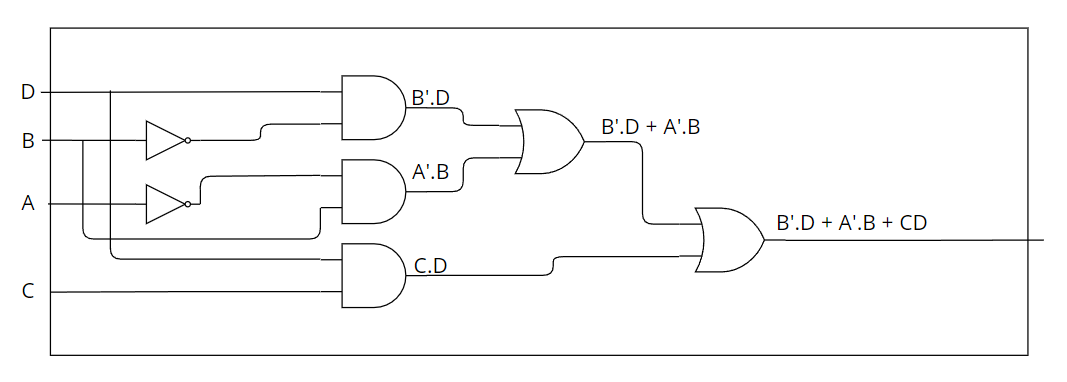
\includegraphics[width=0.9\textwidth]{tp02fig1.png}
    \caption{Circuito para la función $B’D + A’B + CD$}
\end{figure}

\newpage 
\begin{figure}[h]
    \centering
    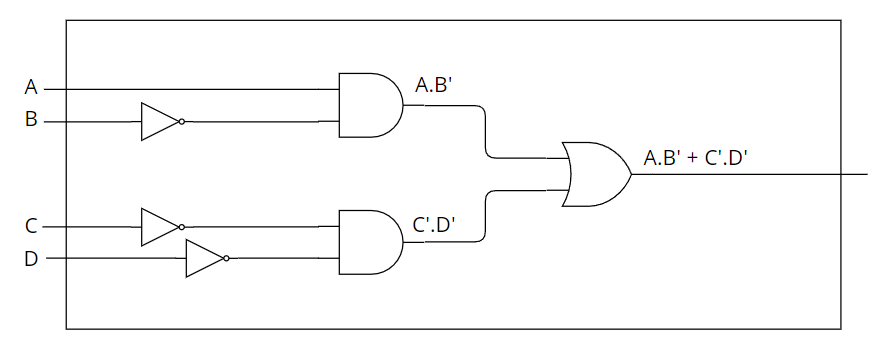
\includegraphics[width=0.9\textwidth]{tp02fig2.png}
    \caption{Circuito para la función $A.B' + C'.D'$}
\end{figure}

\textbf{Punto b)}\\
\begin{itemize}
    \item[b)] $B’.D + A’.B + CD$ para buscar el equivalente con compuertas NAND.\\
    \begin{align*}
        & B’.D + A’.B + CD \\
        &= (B’.D + A’.B + CD)'' \\
        &= ((B'.D)' \cdot (A'.B)' \cdot (C.D)')'
    \end{align*} 
    \item[d)] $A.B' + C'.D'$ para buscar el equivalente con compuertas NAND.\\
    \begin{align*}
        & A.B' + C'.D' \\
        &= (A.B' + C'.D')'' \\
        &= ((A.B')' \cdot (C'.D')')'
    \end{align*}
\end{itemize}

\textbf{Punto c)}\\
\begin{figure}[h]
    \centering
    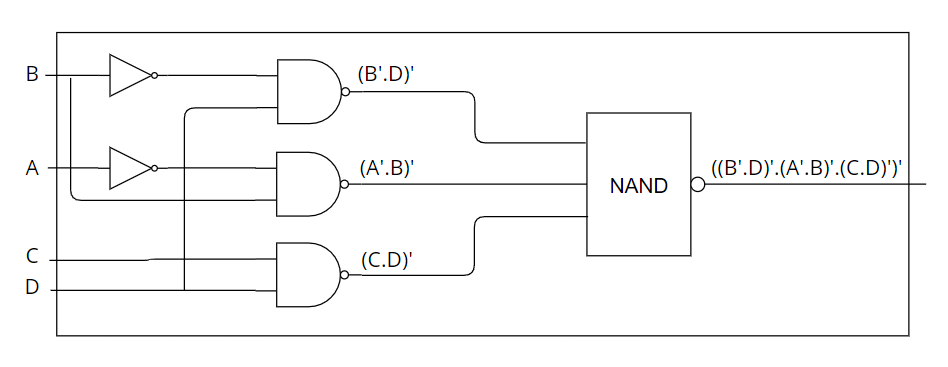
\includegraphics[width=0.9\textwidth]{tp02fig3.png}
    \caption{Circuito para la función $B’.D + A’.B + CD$ con compuertas NAND}
\end{figure}

\newpage
\begin{figure}[h]
    \centering
    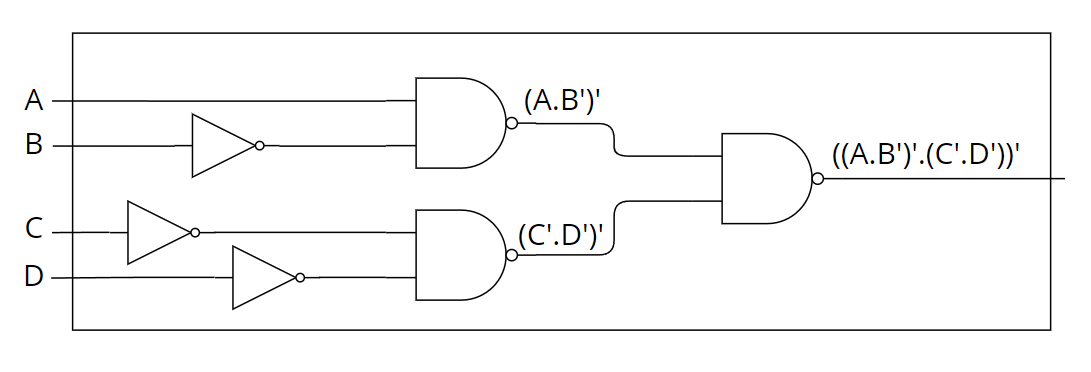
\includegraphics[width=0.9\textwidth]{tp02fig4.png}
    \caption{Circuito para la función $A.B' + C'.D'$ con compuertas NAND}
\end{figure}
\end{solution}

\section*{Ejercicio 3}
La función $OR$-exclusiva, denotada por \^ \ tiene dos entradas y una salida. Si $a$ y $b$ son las entradas y $c$ es la salida, entonces $c$ es $1$ sólo cuando exactamente una de las entradas vale $1$. En el resto de los casos es $0$.
\begin{enumerate}[a)]
    \item Hacer una tabla de verdad de la función $OR$-exclusiva.
    \item Encontrar la expresión equivalente a la función OR-exclusiva utilizando sólo suma de productos y graficar con compuertas.
    \item Implementar una OR-exclusiva de 3 entradas usando OR-exclusivas de 2 entradas.
\end{enumerate}

\begin{solution}
\textbf{Punto a)}\\
La tabla de verdad de la función $OR$-exclusiva es la siguiente:
\begin{table}[H]
    \centering
    \begin{tabular}{|c|c|c|}
    \hline
    $a$ & $b$ & $c$ \\ \hline
    0   & 0   & 0   \\ \hline
    0   & 1   & 1   \\ \hline
    1   & 0   & 1   \\ \hline
    1   & 1   & 0   \\ \hline
    \end{tabular}
\end{table}

\textbf{Punto b)}\\
La expresión equivalente a la función $OR$-exclusiva utilizando sólo suma de productos es:
\begin{align*}
    c &= (a \cdot b') + (a' \cdot b)
\end{align*}
El circuito para la función $OR$-exclusiva es el siguiente:
\begin{figure}[H]
    \centering
    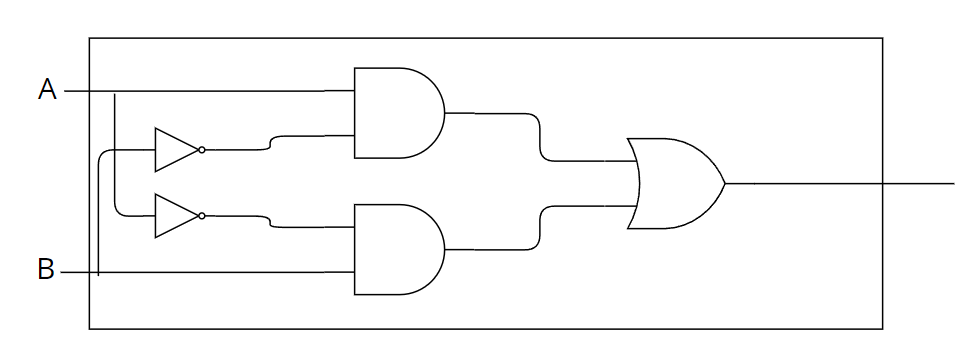
\includegraphics[width=0.7\textwidth]{tp02fig5.png}
    \caption{Circuito para la función $OR$-exclusiva}
\end{figure}

\textbf{Punto c)}\\
La función $OR$-exclusiva de 3 entradas se puede implementar de la siguiente manera:
\begin{figure}[H]
    \centering
    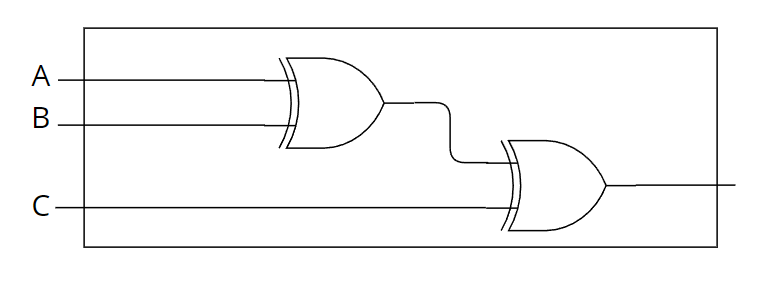
\includegraphics[width=0.7\textwidth]{tp02fig6.png}
    \caption{Circuito para la función $OR$-exclusiva de 3 entradas}
\end{figure}
\end{solution}

\section*{Ejercicio 4}
Mostrar que la función NAND (Not AND) es universal en el sentido de que las funciones NOT, AND, OR y NOR se pueden expresar como productos negados. Graficar las implementaciones de las compuertas NOT, AND, OR y NOR con compuertas NAND.

\begin{solution}
La función NAND es universal en el sentido de que las funciones NOT, AND, OR y NOR se pueden expresar como productos negados.\\

\textbf{NOT:} La función NOT se puede expresar como un producto negado de la siguiente manera:
\begin{figure}[H]
    \centering
    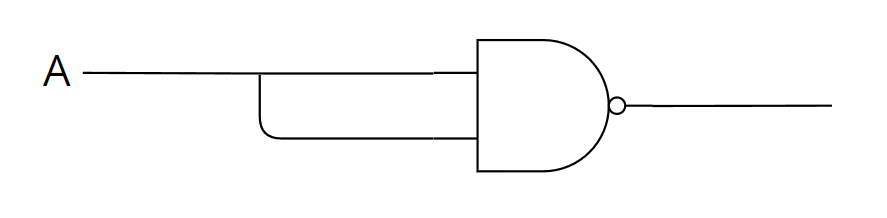
\includegraphics[width=0.3\textwidth]{tp02fig7.png}
    \caption{Circuito para la función NOT con compuertas NAND}
\end{figure}
La tabla de verdad de la función NOT es la siguiente:
\begin{table}[H]
    \centering
    \begin{tabular}{|c|c|}
    \hline
    $a$ & $c$ \\ \hline
    0   & 1   \\ \hline
    1   & 0   \\ \hline
    \end{tabular}
\end{table}

\textbf{AND:} La función AND se puede expresar como un producto negado de la siguiente manera:
\begin{figure}[H]
    \centering
    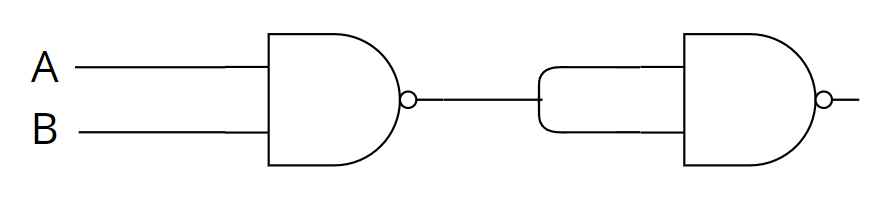
\includegraphics[width=0.3\textwidth]{tp02fig8.png}
    \caption{Circuito para la función AND con compuertas NAND}
\end{figure}
La tabla de verdad de la función AND es la siguiente:
\begin{table}[H]
    \centering
    \begin{tabular}{|c|c|c|}
    \hline
    $a$ & $b$ & $c$ \\ \hline
    0   & 0   & 1   \\ \hline
    0   & 1   & 1   \\ \hline
    1   & 0   & 1   \\ \hline
    1   & 1   & 0   \\ \hline
    \end{tabular}
\end{table}

\textbf{OR:} La función OR se puede expresar como un producto negado de la siguiente manera:
\begin{figure}[H]
    \centering
    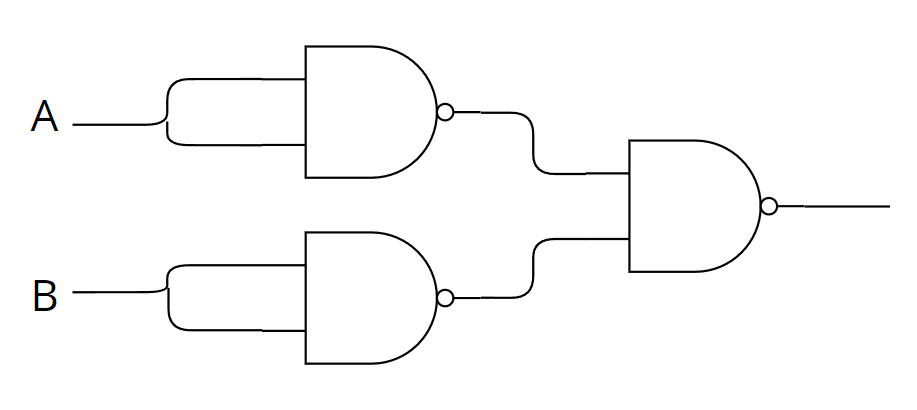
\includegraphics[width=0.3\textwidth]{tp02fig9.png}
    \caption{Circuito para la función OR con compuertas NAND}
\end{figure}
La tabla de verdad de la función OR es la siguiente:
\begin{table}[H]
    \centering
    \begin{tabular}{|c|c|c|}
    \hline
    $a$ & $b$ & $c$ \\ \hline
    0   & 0   & 0   \\ \hline
    0   & 1   & 1   \\ \hline
    1   & 0   & 1   \\ \hline
    1   & 1   & 1   \\ \hline
    \end{tabular}
\end{table}

\textbf{NOR:} La función NOR se puede expresar como un producto negado de la siguiente manera:
\begin{figure}[H]
    \centering
    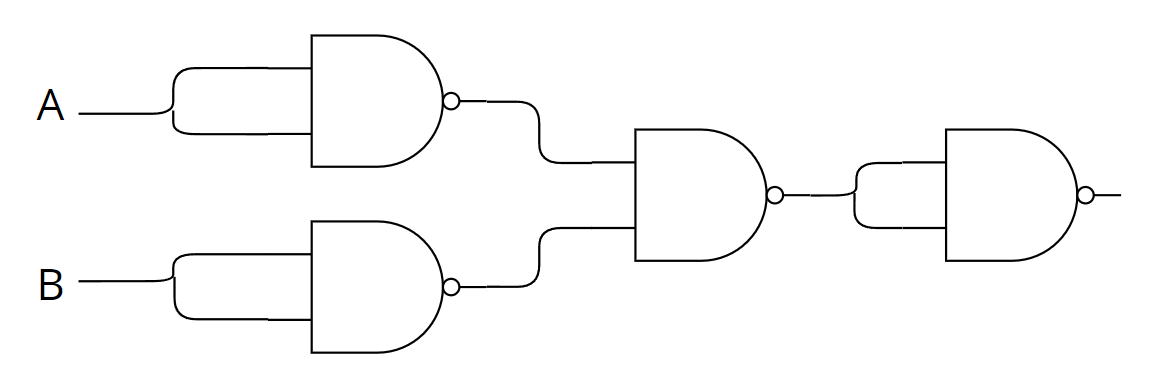
\includegraphics[width=0.3\textwidth]{tp02fig10.png}
    \caption{Circuito para la función NOR con compuertas NAND}
\end{figure}
La tabla de verdad de la función NOR es la siguiente:
\begin{table}[H]
    \centering
    \begin{tabular}{|c|c|c|}
    \hline
    $a$ & $b$ & $c$ \\ \hline
    0   & 0   & 1   \\ \hline
    0   & 1   & 0   \\ \hline
    1   & 0   & 0   \\ \hline
    1   & 1   & 0   \\ \hline
    \end{tabular}
\end{table}
\end{solution}

\section*{Ejercicio 5}
Mostrar que la función NOR (Not OR) es universal en el sentido de que las funciones NOT, OR, AND y NAND se pueden expresar como sumas negadas. Graficar las implementaciones de las compuertas NOT, OR, AND y NAND con compuertas NOR.

\begin{solution}
La función NOR es universal en el sentido de que las funciones NOT, OR, AND y NAND se pueden expresar como sumas negadas.\\

\textbf{NOT:} La función NOT se puede expresar como una suma negada de la siguiente manera:
\begin{figure}[H]
    \centering
    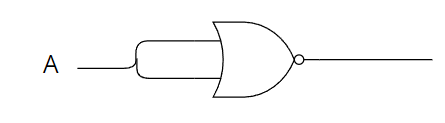
\includegraphics[width=0.3\textwidth]{tp02fig11.png}
    \caption{Circuito para la función NOT con compuertas NOR}
\end{figure}

\textbf{AND:} La función AND se puede expresar como una suma negada de la siguiente manera:
\begin{figure}[H]
    \centering
    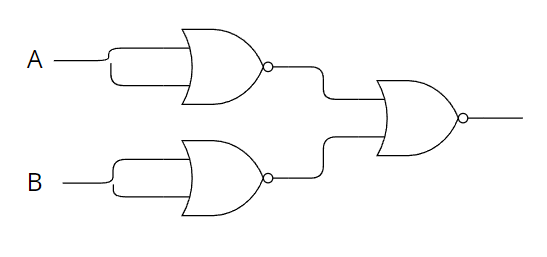
\includegraphics[width=0.3\textwidth]{tp02fig12.png}
    \caption{Circuito para la función AND con compuertas NOR}
\end{figure}

\textbf{OR:} La función OR se puede expresar como una suma negada de la siguiente manera:
\begin{figure}[H]
    \centering
    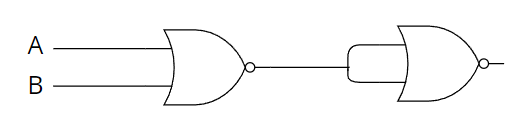
\includegraphics[width=0.3\textwidth]{tp02fig13.png}
    \caption{Circuito para la función OR con compuertas NOR}
\end{figure}

\textbf{NAND:} La función NAND se puede expresar como una suma negada de la siguiente manera:
\begin{figure}[H]
    \centering
    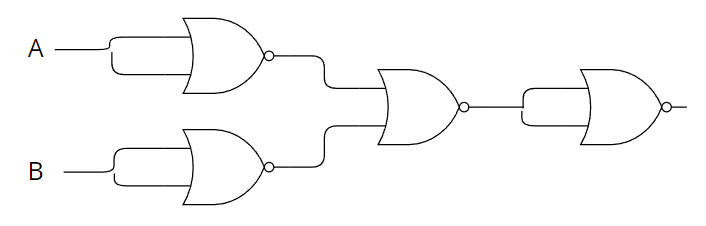
\includegraphics[width=0.3\textwidth]{tp02fig14.png}
    \caption{Circuito para la función NAND con compuertas NOR}
\end{figure}
\end{solution}
\end{document}